\documentclass[11pt]{article}
% THE PREAMBLE
% {

% Packages used.

\usepackage[a4paper, margin=2cm]{geometry} % Allows setting margins.
\usepackage[utf8]{inputenc}   % UTF-8 encoding.
\usepackage[T1]{fontenc} % Font encodings.
\usepackage{titling} % For title formating.
\usepackage{tikz} % For grids.
\usepackage{xcolor} % For colours.
\usepackage{amsmath} % Most math commands.
\usepackage{amssymb} % For math symbols.
\usepackage{enumitem} % For enumerating items.
\usepackage{hyperref} % Linking documents and websites.
\usepackage{import} % Importing ipynb code and other files.
\usepackage{float} % Most often used to stop figures from moving.
\usepackage{tabularx} % More complex tables.
\usepackage[english]{babel}
\usepackage{longtable}
\usepackage{tcolorbox} % For the coloured boxes used in pseudocode.
\usepackage{multicol}
\usepackage{multirow} 
\usepackage[table]{colortbl}
\usepackage{titlesec}
\usepackage{minted} % For code highlights ect.
\usepackage{fontspec}

\setmonofont{DejaVu Sans Mono}[Scale=0.90] % Or Consolas, JetBrains Mono, Source Code Pro, etc.

\emergencystretch 3em
\setlength{\parindent}{0pt} % No indent.
\setlength{\parskip}{10pt} % White space between paragraphs.

% Environment for centering.
% Setting the centering so it doesn't have too much space at the start and end.
\BeforeBeginEnvironment{center}{\setlength{\parskip}{0pt}} 
\AfterEndEnvironment{center}{\setlength{\parskip}{\baselineskip}}

% Environment for mint.
\BeforeBeginEnvironment{minted}{
  \setlength{\parskip}{0pt}
  \setlength{\topsep}{0pt}
  \setlength{\partopsep}{0pt}
}

% Hyperlink settup.
\hypersetup{
    colorlinks=true,    
    urlcolor=black!60!blue,
    citecolor=black!60!blue,
    linkcolor=black!60!blue
}

% Adjusting titles, sections and subsections.
\titlespacing*{\section}{0pt}{2pt}{4pt}  % Adjusts spacing for \section
\titlespacing*{\subsection}{0pt}{3pt}{3pt}  % Adjusts spacing for \subsection
\setlength{\droptitle}{-5em} % Making the title a little higher.
\renewcommand{\maketitle}{%
     \begin{center}
    {\LARGE\bfseries Analyzing Algorithms for the Subset Sum Problem}\\[0.5em]  
    {\large Nina Mislej \hspace{0.9em} \today}\\[0.3em]  
  \end{center}
  \vspace{-1.5em} % Reduce space after title
}

\newcommand{\cpp}{C\raisebox{0.4ex}{\scalebox{0.8}{++}} }

\begin{document}
\maketitle

The entire code can be found on the \href{https://github.com/Edelwy/approximation-algorithms}{\textbf{GitHub repositroy}}. The below mentioned results analyzed and raw can also be found in the repository as well.

\section{Implementation of the Algorithms}

I chose to implement the algorithms in \cpp because it provides sufficient built-in functionality and flexibility, while remaining faster than many other languages. Firstly, here is the implementation of the algorithm used for \textbf{dynamic programming}. The \texttt{memo} table is used for memoization and is initialized to $0$ for every element.

\begin{minted}[fontsize=\fontsize{10.5pt}{11pt}, 
               bgcolor=gray!10, 
               breaklines=true]{cpp}

  bool CSolver::solveDYN( int n, int k, const std::vector<int>& numbers )
  {
      std::vector<std::vector<int>> memo( n, std::vector<int>( k, 0 ) );
      std::function<int( int, int )> solver = [&]( int i, int j ) -> int {
          if( i < 0 || j < 0 || i > n || j > k )
              return std::numeric_limits<int>::min();
  
          if( i == 0 || j == 0 )
              return 0;
  
          auto& mem = memo.at( i - 1 ).at( j - 1 );
          if( mem > 0 ) 
              return mem;
  
          const auto& num = numbers.at( i - 1 );
          mem = std::max( solver( i - 1, j ), solver( i - 1, j - num ) + num );
          return mem;
      };
      auto solution = solver( n, k );
      std::cout << fmt::format( "Solution found was {}.\n", solution );
      return solution == k;
  }
\end{minted}

Next algorithm is the \textbf{exhaustive search}. We do not actually add lists together but keep all elements in one set, which in \cpp is sorted by default.

\begin{minted}[fontsize=\fontsize{10.5pt}{11pt}, 
    bgcolor=gray!10, 
    breaklines=true]{cpp}

  bool CSolver::solveEXH( int n, int k, const std::vector<int>& numbers )
  {
      std::set<int> sums = { 0 };
      for ( int i = 1; i < n; i++ ) {
          auto currSums = sums;
  
          for ( const auto element : currSums ) {
              auto newElement = element + numbers.at( i );
              if ( newElement <= k )
                  sums.insert( newElement );
              if ( newElement == k)
                  break;
          }
      }
      auto solution = *sums.rbegin();
      std::cout << fmt::format( "Maximal element in set is {}.\n", solution );
      return solution == k;
  } 
\end{minted}

\pagebreak
The implementation of the \textbf{greedy algorithm} is optimized by sorting the numbers array first. If we frame this as a maximization problem, we are searching for the maximum sum not exceding $k$. Then this is a $0.5$-approximation, meaning the approximation is at least half as good as the actual solution.

\begin{minted}[fontsize=\fontsize{10.5pt}{11pt}, 
    bgcolor=gray!10, 
    breaklines=true]{cpp}

  bool CSolver::solveGRDY( int n, int k, const std::vector<int>& numbers )
  {
      auto sortedNumbers = numbers;
      std::sort( sortedNumbers.begin(), sortedNumbers.end(), std::greater<int>() );
  
      int solution = 0;
      for ( int i = 0; i < n; i++ ) {
          const auto& element = sortedNumbers.at( i );
          if ( k - solution >= element )
              solution += element;
      }
      auto approx = fmt::format( "Approximation for {} is {}.\n", k, solution );
      approx += fmt::format( "Difference is {}.\n", k - solution );
      std::cout << approx;
      return solution == k;
  }  
\end{minted}

Finally, we have the \textbf{FPTAS algorithm} which is very similar to the exahustive search with addition of trimming the set based on the $\epsilon$ parameter.

\begin{minted}[fontsize=\fontsize{10.5pt}{11pt}, 
    bgcolor=gray!10, 
    breaklines=true]{cpp}

  bool CSolver::solveFPTAS( int n, int k, const std::vector<int>& numbers )
  {
      auto delta = mEpsilon / ( 2 * n );
      std::set<int> sums = { 0 };
      for ( int i = 1; i < n; i++ ) {
          auto tmpSums = sums;
  
          for ( const auto element : tmpSums ) 
              sums.insert( element + numbers.at( i ) );
  
          auto last = *sums.begin();
          tmpSums = { last };
          for ( auto& element : sums ) {
              if( element <= k && element > last * ( 1 + delta ) ) {
                  tmpSums.insert( element );
                  last = element;
              }
              if ( element == k)
                  break;
          }
          sums = tmpSums;
      }
  
      auto solution = *sums.rbegin();
      auto approx = fmt::format( "Approximation for {} is {}. \n", k, solution );
      approx += fmt::format( "The epsilon value was {}.", mEpsilon );
      approx += fmt::format( "Difference is {}.\n", k - solution );
      std::cout << approx;
      return solution == k;
  }  
\end{minted}

Which algorithm is used is parsed from parameters and decided based on the enum value.

\begin{minted}[fontsize=\fontsize{10.5pt}{11pt}, 
    bgcolor=gray!10, 
    breaklines=true]{cpp}
  enum class EMode { DYN = 1, EXH = 2, GRDY = 3, FPTAS = 4 };
\end{minted}

\pagebreak

\section{Testing on Public Test Cases}

Firstly let us examine the performance of all four algorithms for the public test cases provided in \href{https://ucilnica.fri.uni-lj.si/mod/assign/view.php?id=32883}{spletna učilnica}. I implemented a \texttt{Benchmark} class available in the repository that times the performance. The $\epsilon$ value was $0.2$ for the fourth algorithm. There exists a \textbf{feasable folution} for every test case. 

\begin{figure}[!hbpt]
    \begin{minipage}{0.64\textwidth}
        \begin{table}[H]
            \centering
            \begin{tabular}{|l|c|c|c|c|} \hline
                \cellcolor{blue!20} & \multicolumn{4}{c|}{\cellcolor{blue!20}\texttt{time}} \\ \cline{2-5}
                \cellcolor{blue!20} \texttt{test} & \texttt{DYN} & \texttt{EXH} & \texttt{GRDY} & \texttt{FPTAS} \\ \hline
                \makecell[l]{ \texttt{n = 100} \\ \texttt{k = 200}} & 0.00003 & 0.00362 & 0.00001 & \cellcolor{red!20}{0.00895} \\ \hline
                \makecell[l]{ \texttt{n = 50} \\ \texttt{k = 200000}} & 0.00992 & \cellcolor{red!20}{1.14751} & 0.00001 & 0.02338 \\ \hline
                \makecell[l]{ \texttt{n = 500} \\ \texttt{k = 2000}} & 0.00020 & 0.25861 & 0.00006 & \cellcolor{red!20}{0.60971} \\ \hline
                \makecell[l]{ \texttt{n = 40} \\ \texttt{k = 1230000}} & 0.04424 & \cellcolor{red!20}{7.79745} & 0.00001 & 0.01751 \\ \hline
                \makecell[l]{ \texttt{n = 1000} \\ \texttt{k = 72000}} & 0.06364 & \cellcolor{red!20}{25.26750} & 0.00013 & 21.36842 \\ \hline
            \end{tabular}
            \caption{Time in seconds for the public test cases.}
        \end{table}
    \end{minipage}
    \begin{minipage}{0.35\textwidth}
        \begin{table}[H]
            \centering
            \begin{tabular}{|l|c|c|} \hline
                \cellcolor{blue!20} & \multicolumn{2}{c|}{\cellcolor{blue!20}\texttt{difference}} \\ \cline{2-3}
                \cellcolor{blue!20} \texttt{test} & \texttt{GRDY} & \texttt{FPTAS} \\ \hline
                \makecell[l]{ \texttt{n = 100} \\ \texttt{k = 200}}  & \cellcolor{red!20}{4} & 0 \\ \hline
                \makecell[l]{ \texttt{n = 50} \\ \texttt{k = 200000}} &  \cellcolor{red!20}{19516} & 337 \\ \hline
                \makecell[l]{ \texttt{n = 500} \\ \texttt{k = 2000}} &  \cellcolor{red!20}{34} & 0 \\ \hline
                \makecell[l]{ \texttt{n = 40} \\ \texttt{k = 1230000}} &  \cellcolor{red!20}{33687} & 4 \\ \hline
                \makecell[l]{ \texttt{n = 1000} \\ \texttt{k = 72000}} & \cellcolor{red!20}{897} & 7 \\ \hline
            \end{tabular}
            \caption{Difference from $k$.}
        \end{table} 
    \end{minipage}  
\end{figure}

The red cells represent the longest running time. The first case was easily solveble by all algorithms with time being \textbf{under a second}. The \textbf{dynamic programming} approach performed drastically better than the \textbf{exhaustive search} in terms of finding an optimal solution. It even performed better than the \textbf{FPTAS} algorithm in most cases. While the greedy algorithm performed better timewise, it did perform a lot worse in terms of approximation.

\section{Test Case Generation for Hard Scenarios}

Let us concentrate on challenging examples for each algorithm we implemented.

\textbf{Case 1:} One hard case for dynamic programming arises when the input list consists entirely of very small values, such as \textbf{all ones}. In this situation, the algorithm makes only minimal progress in both the index and sum dimensions. As a result, the algorithm is forced to explore almost the entire $n \times k$ table. This is expecially important when $k$ is large. 

\textbf{Case 2:} Another difficult example for dynamic programming arises when determining that no solution exists in a very large $n \times k$ table, even in trivial cases. Suppose we choose a relatively large $k$ and a list of numbers whose \textbf{total sum is less than} $k$, making it impossible to reach the target. In such cases, the algorithm still allocates the full table and explores many combinations before ultimately concluding that no solution exists. 

\textbf{Case 3:} Both cases mentioned above are difficult for the \textbf{exahustive search} as well as there rarely any filtering and the list becomes very large. Since we are working with set that should not be an issue. We can modify the second case in a way that every sum of arbitrary elements from the list is unique. We can achieve this by taking powers of $2$ as the initial list, mimicking binary representation. 

\textbf{Case 4:} Now we discuss cases where approximation algorithms produce very bad results. One such case for the \textbf{greedy algorithm without sorting} would be having just two elements $1$ and $2000$ and $k$ being $2000$ perhaps. The best possible solution would of course be $2000$ however the approximation will be $0$. Just to keep $n$ consistent with the other cases, we will add some padding with zeros. Since we implemented sorting the difference is actually $49$.

\textbf{Case 5:} We can however still find a case where we achieve the \textbf{worst possible value}. If we take the numbers  in the inital list to be $51, 50, 50$ and set $k$ to $100$ we would get $51$ which is a $1$ over half the optimal value. We can generate more generic test cases like this for arbitrary $k$. Take the largest element of the list to be $\lceil \frac{k}{2} \rceil + 1$ and all other elements $\frac{k}{2}$.

\textbf{Case 6:} Since \textbf{FPTAS} only keeps the sum if it is greater than $1 + \frac{\epsilon}{2n}$ we can make the trimming process inefficient by creating elements who are only slightly larger than the previous one, keeping them under this limit. We do this by taking $a_i = \lfloor \frac{k}{n \cdot (1 + \epsilon)} \rfloor + i$ as the $i$-th element in the initial list. 

\begin{figure}[!hbpt]
    \begin{minipage}{0.6\textwidth}
        \begin{table}[H]
            \centering
            \begin{tabular}{|c|l|c|c|c|c|} \hline
                \cellcolor{blue!20} & \cellcolor{blue!20} &  \multicolumn{4}{c|}{\cellcolor{blue!20}\texttt{time}} \\ \cline{3-6} 
                \cellcolor{blue!20} & \cellcolor{blue!20}\texttt{parameters} & \texttt{DYN} & \texttt{EXH} & \texttt{GRDY} & \texttt{FPTAS} \\ \hline
                1 & \makecell[l]{ \texttt{n = 50000} \\ \texttt{k = 45000}} & 0.0181 & 3.254 & 0.001 & 8.022 \\ \hline
                2 & \makecell[l]{ \texttt{n = 5000} \\ \texttt{k = 103348}} & 0.598 & 95.076 & 0.001 & 209.657 \\ \hline
                3 & \makecell[l]{ \texttt{n = 25} \\ \texttt{k = 33554432}} & 0.841 & 11.800 & 0.000 & 0.017 \\ \hline
            \end{tabular}
            \caption{Time in seconds for the generated test cases.}
        \end{table} 
    \end{minipage}
    \begin{minipage}{0.39\textwidth}
        \begin{table}[H]
            \centering
            \begin{tabular}{|c|l|c|c|} \hline
                \cellcolor{blue!20} & \cellcolor{blue!20} & \multicolumn{2}{c|}{\cellcolor{blue!20}\texttt{difference}} \\ \cline{3-4}
                \cellcolor{blue!20} & \cellcolor{blue!20} \texttt{test} & \texttt{GRDY} & \texttt{FPTAS} \\ \hline
                2 & \makecell[l]{ \texttt{n = 2} \\ \texttt{k = 2000}} & 1 & 107 \\ \hline
                3 & \makecell[l]{ \texttt{n = 2} \\ \texttt{k = 2000}} & 1 & 95764 \\ \hline
                5 & \makecell[l]{ \texttt{n = 3} \\ \texttt{k = 100}} & 49 & 0 \\ \hline
                6 & \makecell[l]{ \texttt{n = 100} \\ \texttt{k = 200}} & 0 & 0 \\ \hline
            \end{tabular}
            \caption{Difference from $k$.}
        \end{table} 
    \end{minipage}
\end{figure}

Test cases $2$ and $3$ do not have a feasable solution while the rest do.

\section{Epsilon Impact on Runtime}

To test the importance of the $\epsilon$ parameter for the \textbf{FPTAS runtime}, the algorithm was tested on the third public test case. The testing started at $\epsilon$ being $0.0$ and ended with epsilon $3.0$ with the $0.1$ being the increasing step.

\begin{figure}[h!]
    \centering
    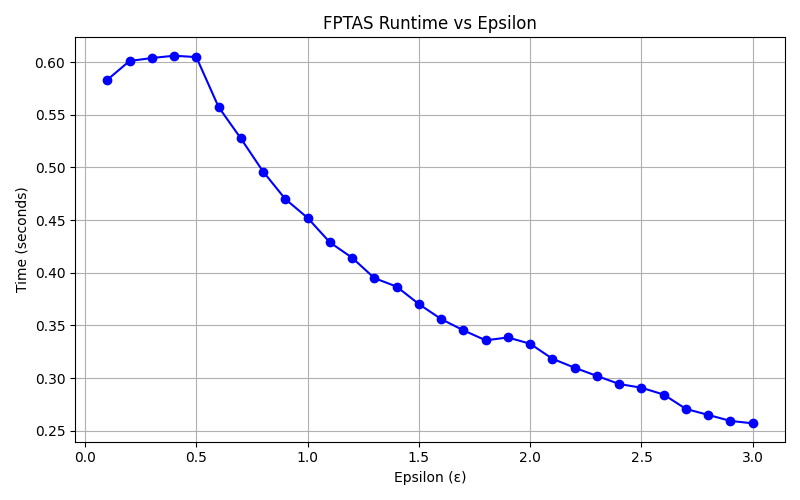
\includegraphics[width=0.7\textwidth]{plot.png} 
    \caption{The Importance of Epsilon for Time Complexity}
    \label{fig:epsilon_vs_time}
\end{figure}

\end{document}